\documentclass[a4paper, 12pt]{article}
\usepackage[utf8]{inputenc}
\usepackage[T1]{fontenc}
\usepackage[french]{babel}
\usepackage{graphicx}
\usepackage{amsmath}
\usepackage{verbatim}
\usepackage{array}
\usepackage{amssymb}
\usepackage{hyperref}
\usepackage[linesnumbered, french, boxed]{algorithm2e}
\usepackage{forest}
\usepackage{pdfpages}

\author{Mickael GAULT}
\title{}
\date{\today}

\begin{document}
\maketitle
\newpage
\tableofcontents
\newpage
\section{Sujet}
Le site est basé en 2 parties indépendantes. Une partie dédiée aux chefs/cheftaines et celle dédiée aux jeunes.
\subsection{Principe et motivations}
Le site se base sur la pédagogie (méthode d'éducation) Scout/Guide des Scouts et Guides de France\footnote{Toutes les informations appartiennent aux SGDF : \url{http://sgdf.fr}}. Pour ce site, l'enjeu est de proposer aux jeunes SG une façon d'explorer les outils pédagogiques mis à leur disposition de façon interactive. Les chefs/cheftaines pourront également explorer la pédagogie SG mais de façon plus directe. En annexe, se trouve la présentation officielle des propositions pédagogiques chez les SGDF.
\subsection{Partie chefs/cheftaines}
Les chefs/cheftaines pourront travailler la nouvelle pédagogie\footnote{En effet, elle est actuellement en déploiement en remplacement de l'ancienne(travail de la DG et du CA depuis 2020)} avec des fiches synthèses et un lien vers les ressources des jeunes. Les chefs pourront également partager des fichiers et choisir si ils veulent rendre celui-ci public ou privé. Il est possible de contacter le propriétaire du site et d'en savoir plus grâce à la page \verb+about+.
\subsection{Partie jeunes}
 Les jeunes exploreront les différents pages en se posant des questions :
\begin{figure}[!h]
  \center
  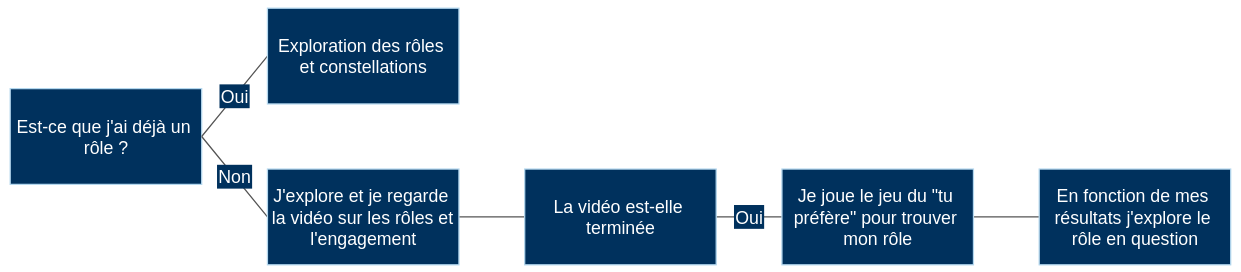
\includegraphics[scale=0.3]{decision_tree.png}
\end{figure}
\section{Plan du site}
\begin{forest}
  for tree={
    font=\ttfamily,
    grow'=0,
    child anchor=west,
    parent anchor=south,
    anchor=west,
    calign=first,
    edge path={
      \noexpand\path [draw, \forestoption{edge}]
      (!u.south west) +(7.5pt,0) |- node[fill,inner sep=1.25pt] {} (.child anchor)\forestoption{edge label};
    },
    before typesetting nodes={
      if n=1
        {insert before={[,phantom]}}
        {}
    },
    fit=band,
    before computing xy={l=15pt},
  }
[index.php
  [chef.php
    [parcourir.php]
    [contact.php]
    [about.php]
    [password.php]
    [register.php]
    [profil.php
      [myfiles.php]
      [options.php]
      [user\_browser.php]
    ]
    [ressources.php]
  ]
  [accueil.html
    [liste.php]
    [video.html
      [questionnaire.html
        [resultat.php]
      ]
    ]
  ]
]
\end{forest}
\section{Fonctionnalités}
Chaque utilisateur peut enregistrer des fichiers pdf dans sont espace personnel, il peut choisir sir le fichier est public (accessible à tous) ou privé. Tous les fichiers publics sont accessibles soit par l'espace personnel de l'utilisateur soit par l'onglet \verb+parcourir+. Il peut également supprimer ses propres fichiers. L'administrateur peut supprimer et voir tous les fichiers. L'administrateur peut également supprimer des utilisateurs. Tout le monde à accès aux fichiers publics.
\section{Base de données}
La base de données est en réalité en 2 parties :
\begin{itemize}
\item Pour la pédagogie pure
\item Pour la gestion du site
\end{itemize}
\subsection{Partie : pédagogie} 
\begin{verbatim}
ROLES

cid         name        type         notnull     dflt_value  pk        
----------  ----------  ----------   ----------  ----------  ----------
0           idRole      INT          0                       1         
1           nom         VARCHAR(20)  0                       0        

CONSTELLATIONS

cid         name        type         notnull     dflt_value  pk        
----------  ----------  ----------   ----------  ----------  ----------
0           idConst     INT          0                       1         
1           nom         VARCHAR(50)  0                       0         
2           couleur     TEXT         0                       0      

LIEN

cid         name        type          notnull     dflt_value  pk        
----------  ----------  ----------    ----------  ----------  ----------
0           idRole      INT           0                       1         
1           idConst     INT           0                       2         
2           descriptio  VARCHAR(255)  0                       0         
3           exemples    TEXT          0                       0      
\end{verbatim}
La table \verb+ROLES+ contient les 6 rôles, la table \verb+CONSTELLATIONS+ contient les 6 constellations ainsi qu'un code hexadécimal représentant une couleur et la table \verb+lien+ contient une description et des exemples (séparés par des virgules) pour chaque binome (role,constellation), on parle ici d'un produit cartésien des identifiants de roles et de constellations\footnote{de (1,1) à (6,6)}
\subsection{Partie : Administration}
\begin{verbatim}
USER

id         name        type           notnull     dflt_value  pk        
----------  ----------  ----------    ----------  ----------  ----------
0           id          INTEGER       0                       1         
1           name        VARCHAR(255)  1                       0         
2           password    VARCHAR(255)  1                       0         
3           statut      TEXT          1           'restricte  0         

FILES

cid         name        type          notnull     dflt_value  pk        
----------  ----------  ----------    ----------  ----------  ----------
0           idF         INTEGER       0                       1         
1           name        VARCHAR(255)  0                       0         
2           visibility  INTEGER       1           0           0      

POSSESS

cid         name        type        notnull     dflt_value  pk        
----------  ----------  ----------  ----------  ----------  ----------
0           idF         INTEGER     0                       1         
1           idU         INTEGER     0                       2    
\end{verbatim}
La table \verb+USER+ contient le nom, le mot de passe et le statut (qui est soit 0 soit 1). Ce dernier permet de différencier les utilisateurs lambda des administrateurs. la table \verb+FILES+ contient le nom (le nom du fichier.pdf) et sa visibilité (0 pour privé et 1 pour public). La table \verb+POSSESS+ permet de dire qu'un fichier est accessible à un utilisateur. Un fichier peut appartenir à plusieurs utilisateurs\footnote{Dans le cas où un utilisateur ajoute un fichier existant}.
\newpage
\section*{Annexe}
\addcontentsline{toc}{section}{Annexe} 
\subsection*{Lexique}
  \addcontentsline{toc}{subsection}{Lexique}
\begin{tabular}{rl}
  SGDF & Scouts et Guides de France\\
  F & Farfadets (6-8 ans)\\
  LJ & Louveteaux et Jeannettes (8-11 ans)\\
  SG & Scouts et Guides (11-14 ans)\\
  PC & Pionniers et Caravelles (14-17 ans)\\
  Compa & Compagnons (17-19 ans)\\
  CA & Conseil d'Administration\\
  DG & Délégation Générale\\
  Chef & Equivalent d'animateur aux SGDF\\
  Cheftaine & Féminin de chef\\
\end{tabular}
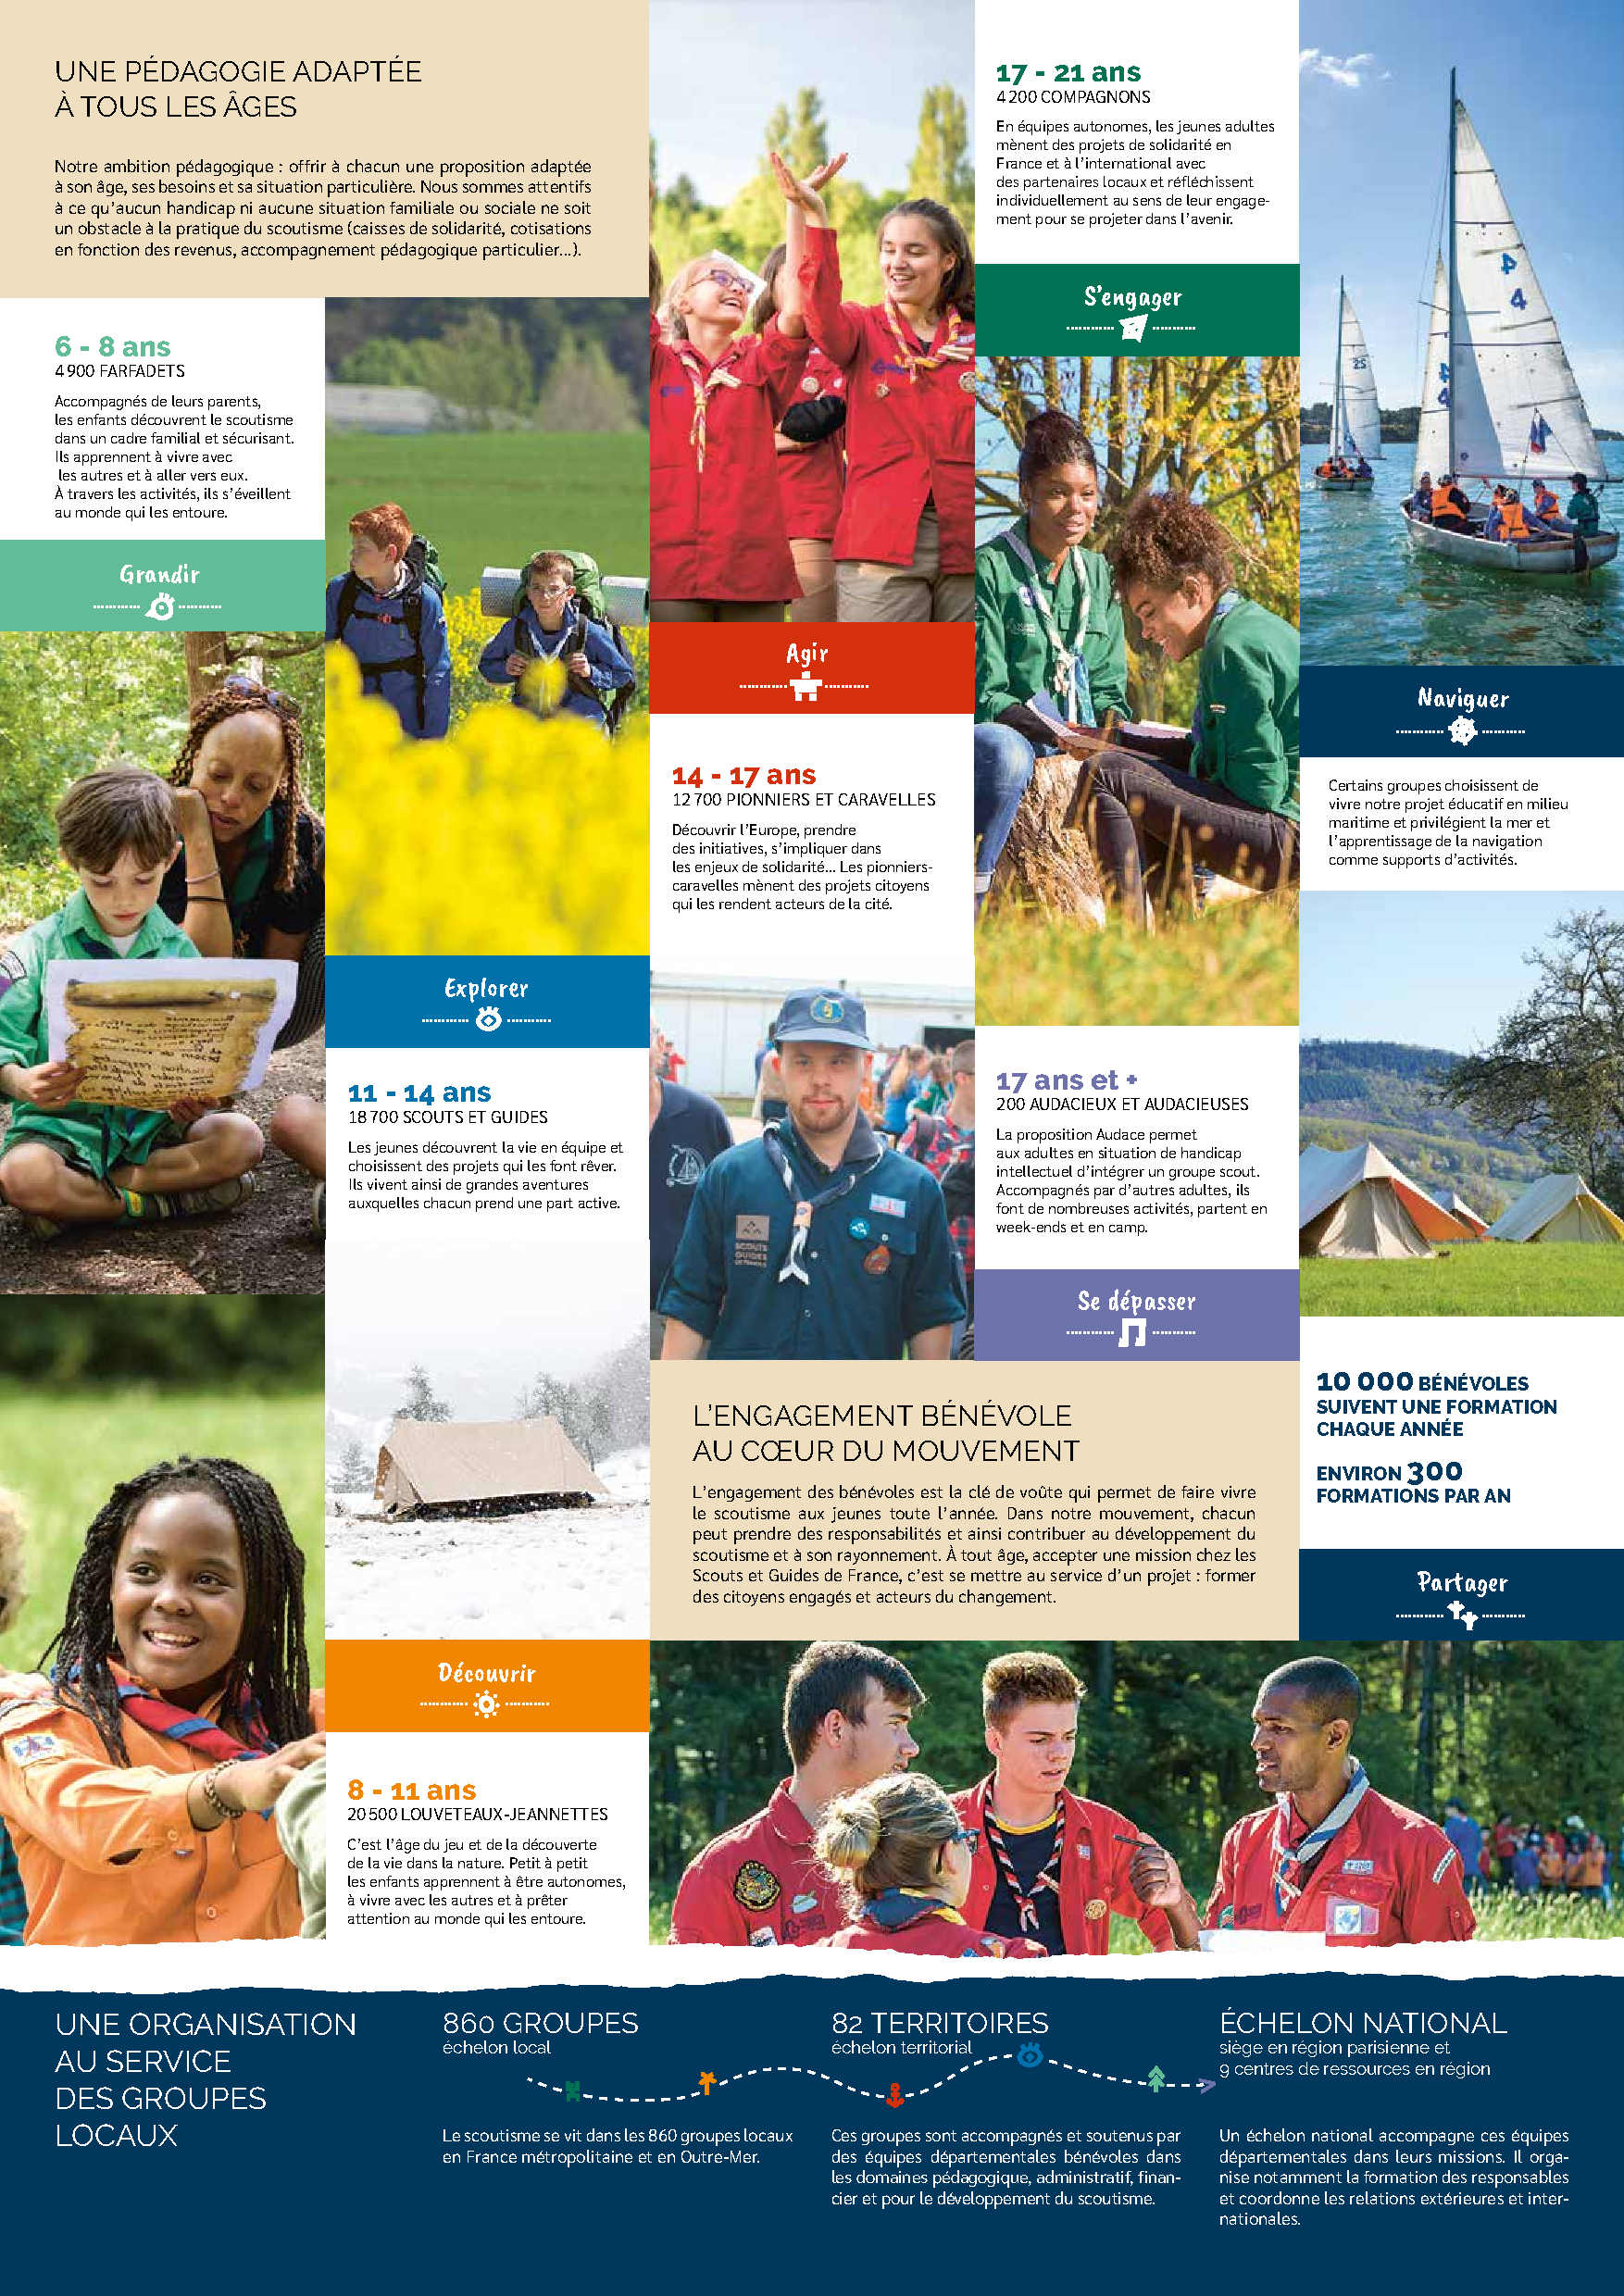
\includepdf[pages=-]{ages.pdf}  
\end{document}   